\documentclass[12pt]{article}

% Packages
\usepackage{amsmath, amssymb, mathtools}
\usepackage{graphicx}
\usepackage{physics}
\usepackage{geometry}
\usepackage{enumitem}
\usepackage{bm}
\usepackage{listings}
\usepackage{xcolor}
\usepackage{float}

% Geometry settings
\geometry{letterpaper, margin=1in}
\setlength{\parindent}{0pt}

\definecolor{codegreen}{rgb}{0,0.6,0}
\definecolor{codegray}{rgb}{0.5,0.5,0.5}
\definecolor{codepurple}{rgb}{0.58,0,0.82}
\definecolor{backcolour}{rgb}{0.95,0.95,0.92}

\lstdefinestyle{mystyle}{
    backgroundcolor=\color{backcolour},   
    commentstyle=\color{codegreen},
    keywordstyle=\color{magenta},
    numberstyle=\tiny\color{codegray},
    stringstyle=\color{codepurple},
    basicstyle=\ttfamily\footnotesize,
    breakatwhitespace=false,         
    breaklines=true,                 
    captionpos=b,                    
    keepspaces=true,                 
    numbers=left,                    
    numbersep=5pt,                  
    showspaces=false,                
    showstringspaces=false,
    showtabs=false,                  
    tabsize=2
}

\lstset{style=mystyle}

% Title
\title{Butterworth Filter Design}
\author{Sanjot Bains}
\date{\today}

\begin{document}

\maketitle

% ----------------------
\section*{Introduction}
The objective of this assignment is to construct a simple program for the design of analog lowpass Butterworth filters. The program takes as input the standard design specifications:
\begin{itemize}
    \item Passband frequency ($\omega_p$)
    \item Maximum passband attenuation ($a_{max}$)
    \item Stopband frequency ($\omega_s$)
    \item Minimum stopband attenuation ($a_{min}$)
\end{itemize}
We test the program with the following specifications:
\begin{itemize}
    \item Passband frequency: $\omega_p = 5\text{k rad/s}$
    \item Max. passband attenuation: $a_{max} = 0.5\ \text{dB}$
    \item Stopband frequency: $\omega_s = 10\text{k rad/s}$
    \item Min. stopband attenuation: $a_{min} = 20\ \text{dB}$
\end{itemize}
The results include:
\begin{enumerate}
    \item The order of the filter
    \item Cutoff frequency $\omega_c$
    \item Locations of the poles
    \item The transfer function
    \item Frequency-response plot (amplitude only)
    \item Verification of the design at passband and stopband frequencies
\end{enumerate}

\section*{Design Specifications}
\begin{lstlisting}[language=Matlab, caption={Design Specifications}]
% Passband Frequency:
omega_p = 5000;     % rad/s
% Maximum Passband Attenuation:
a_max = 0.5;        % dB
% Stopband Frequency:
omega_s = 10_000;   % rad/s
% Minimum Stopband Attenuation:
a_min = 20;         % dB
\end{lstlisting}

\section*{Step 1: Filter Order}
The order $n$ of the filter is given by:
\begin{equation*}
n \geq \frac{ \log_{10} \left( \frac{10^{a_{min}/10} - 1}{10^{a_{max}/10} - 1} \right) }{ 2 \log_{10} (\omega_s/\omega_p) }
\end{equation*}

\begin{lstlisting}[language=Matlab, caption={Order Calculation}]
numerator = log10(
        (10^(a_min / 10) - 1) ...
      / (10^(a_max / 10) - 1)
    );
denominator = 2 * log10(omega_s / omega_p);

n = ceil(numerator / denominator); % Filter Order
    %   = 5
\end{lstlisting}
Thus, the filter order is $n = 5$.

\section*{Step 2: Cutoff Frequency}
The cutoff frequency $\omega_c$ must satisfy:
\begin{equation*}
\frac{\omega_p}{(10^{a_{max}/10} - 1)^{1/(2n)}} \leq \omega_c \leq \frac{\omega_s}{(10^{a_{min}/10} - 1)^{1/(2n)}}
\end{equation*}
\begin{lstlisting}[language=Octave, caption={Cutoff Frequency Calculation}]
min_omega_c =   omega_p / (
                (10^(a_max / 10) - 1)^(1 / (2*n))
            ); %    = 6170.6 rad/s
max_omega_c =   omega_s / (
                (10^(a_min / 10) - 1)^(1 / (2*n))
            ); %    = 6315.9 rad/s

omega_c = 6200;    % Chosen Cutoff Frequency
\end{lstlisting}
We choose $\omega_c = 6200\ \text{rad/s}$.


\section*{Step 3: Poles of the Transfer Function}
For $n=5$ (odd), the poles are:
\begin{equation*}
s_k = \omega_c \exp\left( j \frac{2k\pi}{2n} \right), \quad k = 0, 1, ..., 2n-1
\end{equation*}

We select the $n$ poles in the left-half plane:
\begin{lstlisting}[language=Matlab, caption={Poles Calculation}]
k = 0:(2*n - 1);
s = omega_c * exp( j * k * pi / n );
% The left-half plane is distinguished by the real part of s being negative
s_left = s(real(s) < 0);
\end{lstlisting}
The poles are:
\begin{align*}
&-1915.9 + 5896.6j \\
&-5015.9 + 3644.3j \\
&-6200.0 + 0.0j \\
&-5015.9 - 3644.3j \\
&-1915.9 - 5896.6j
\end{align*}
\begin{figure}[H]
    \centering
    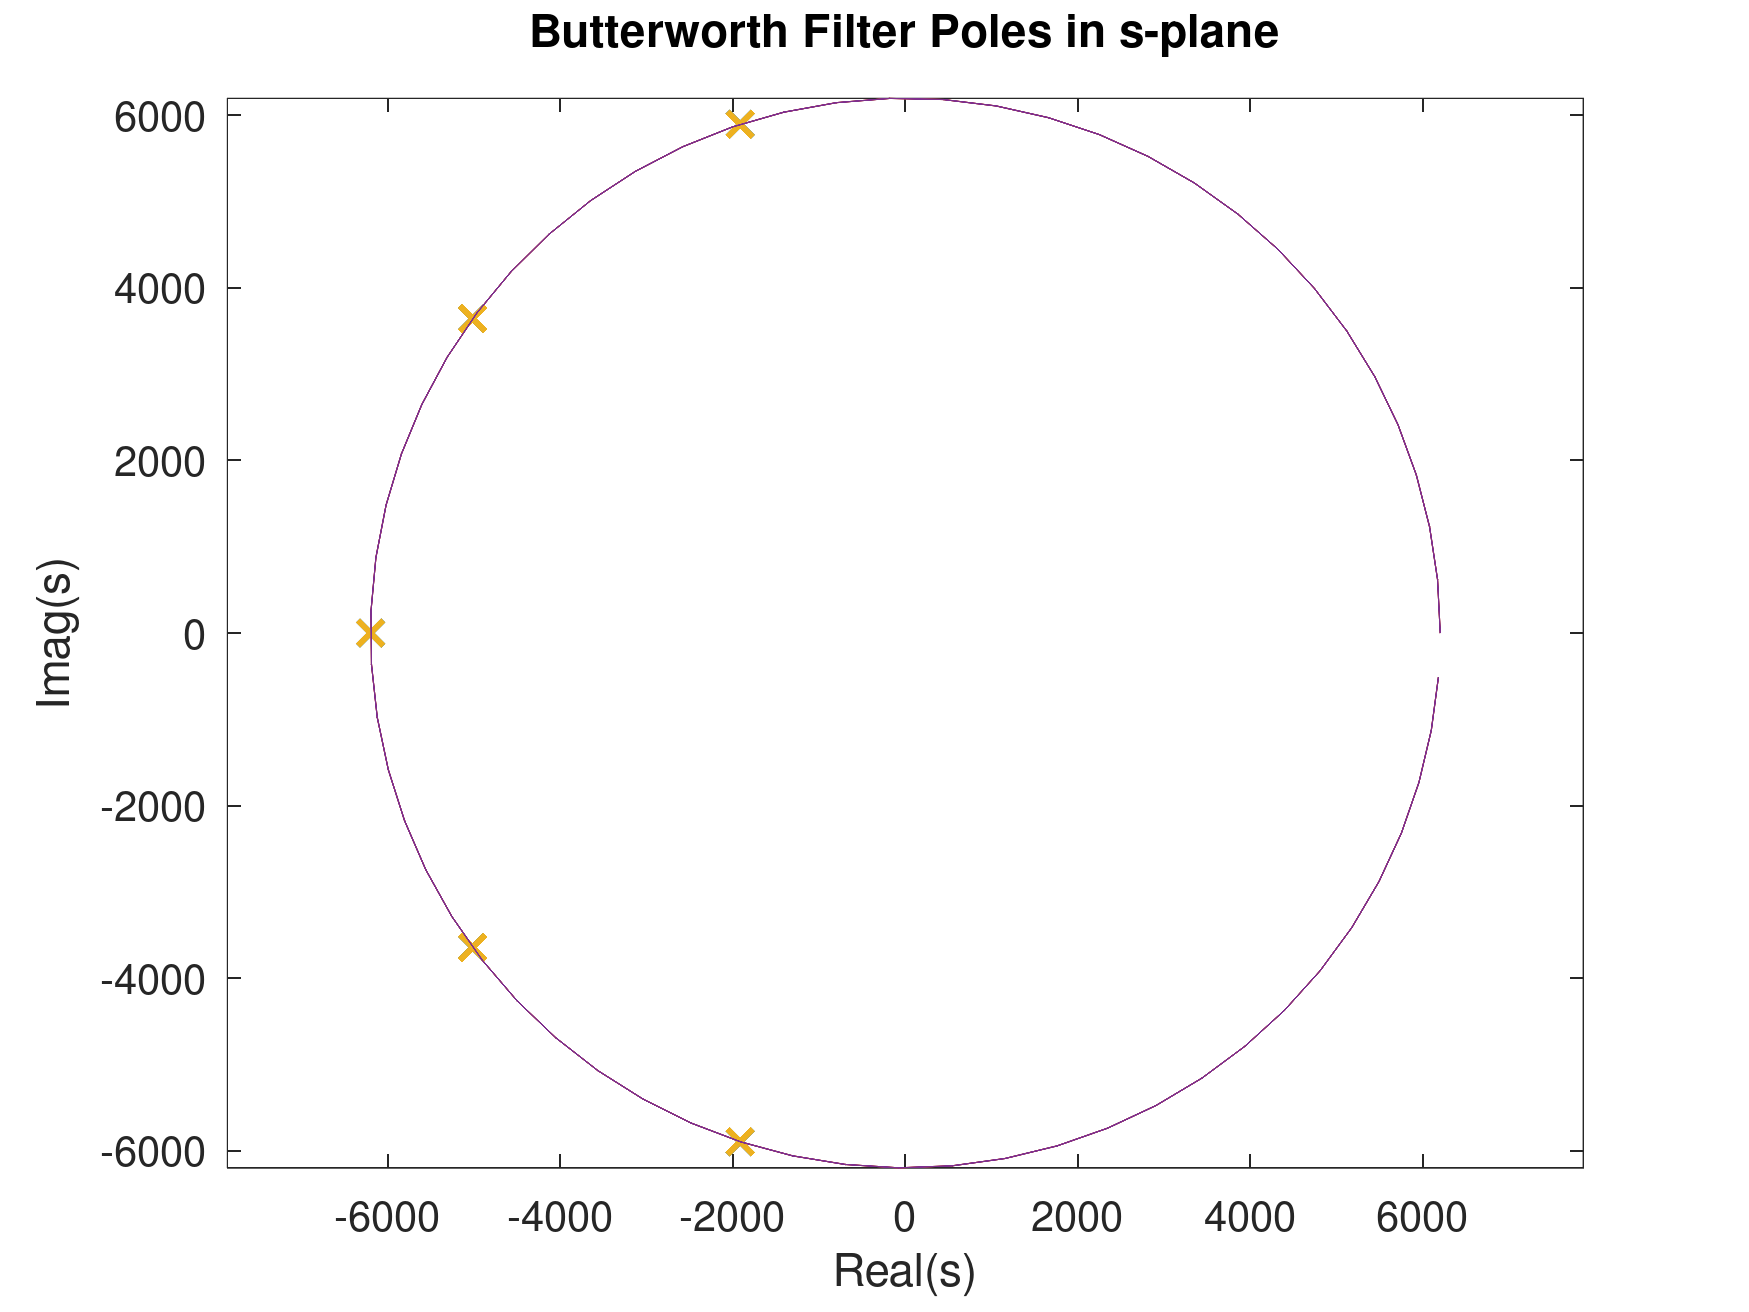
\includegraphics[width=0.5\textwidth]{filter_poles.png}
    \caption{Butterworth Filter Poles in s-plane}
\end{figure}

\section*{Step 4: Transfer Function}
The transfer function is:
\begin{equation*}
H_n(s) = \frac{\omega_c^n}{(s - s_1)(s - s_2)\cdots(s - s_n)}
\end{equation*}

\begin{lstlisting}[language=Matlab, caption={Transfer Function}]
H_n = @(omega) omega_c^n ./ prod(bsxfun(@minus, j*omega(:), s_left), 2);
\end{lstlisting}

\section*{Frequency Response}
The frequency response is computed and plotted:
\begin{lstlisting}[language=Matlab, caption={Frequency Response Plot}]
freq_range = linspace(1, 25000); %  rad/s
freq_response = H_n(freq_range); 
freq_response_dB = 20*log10(abs(freq_response));
\end{lstlisting}
\begin{figure}[H]
    \centering
    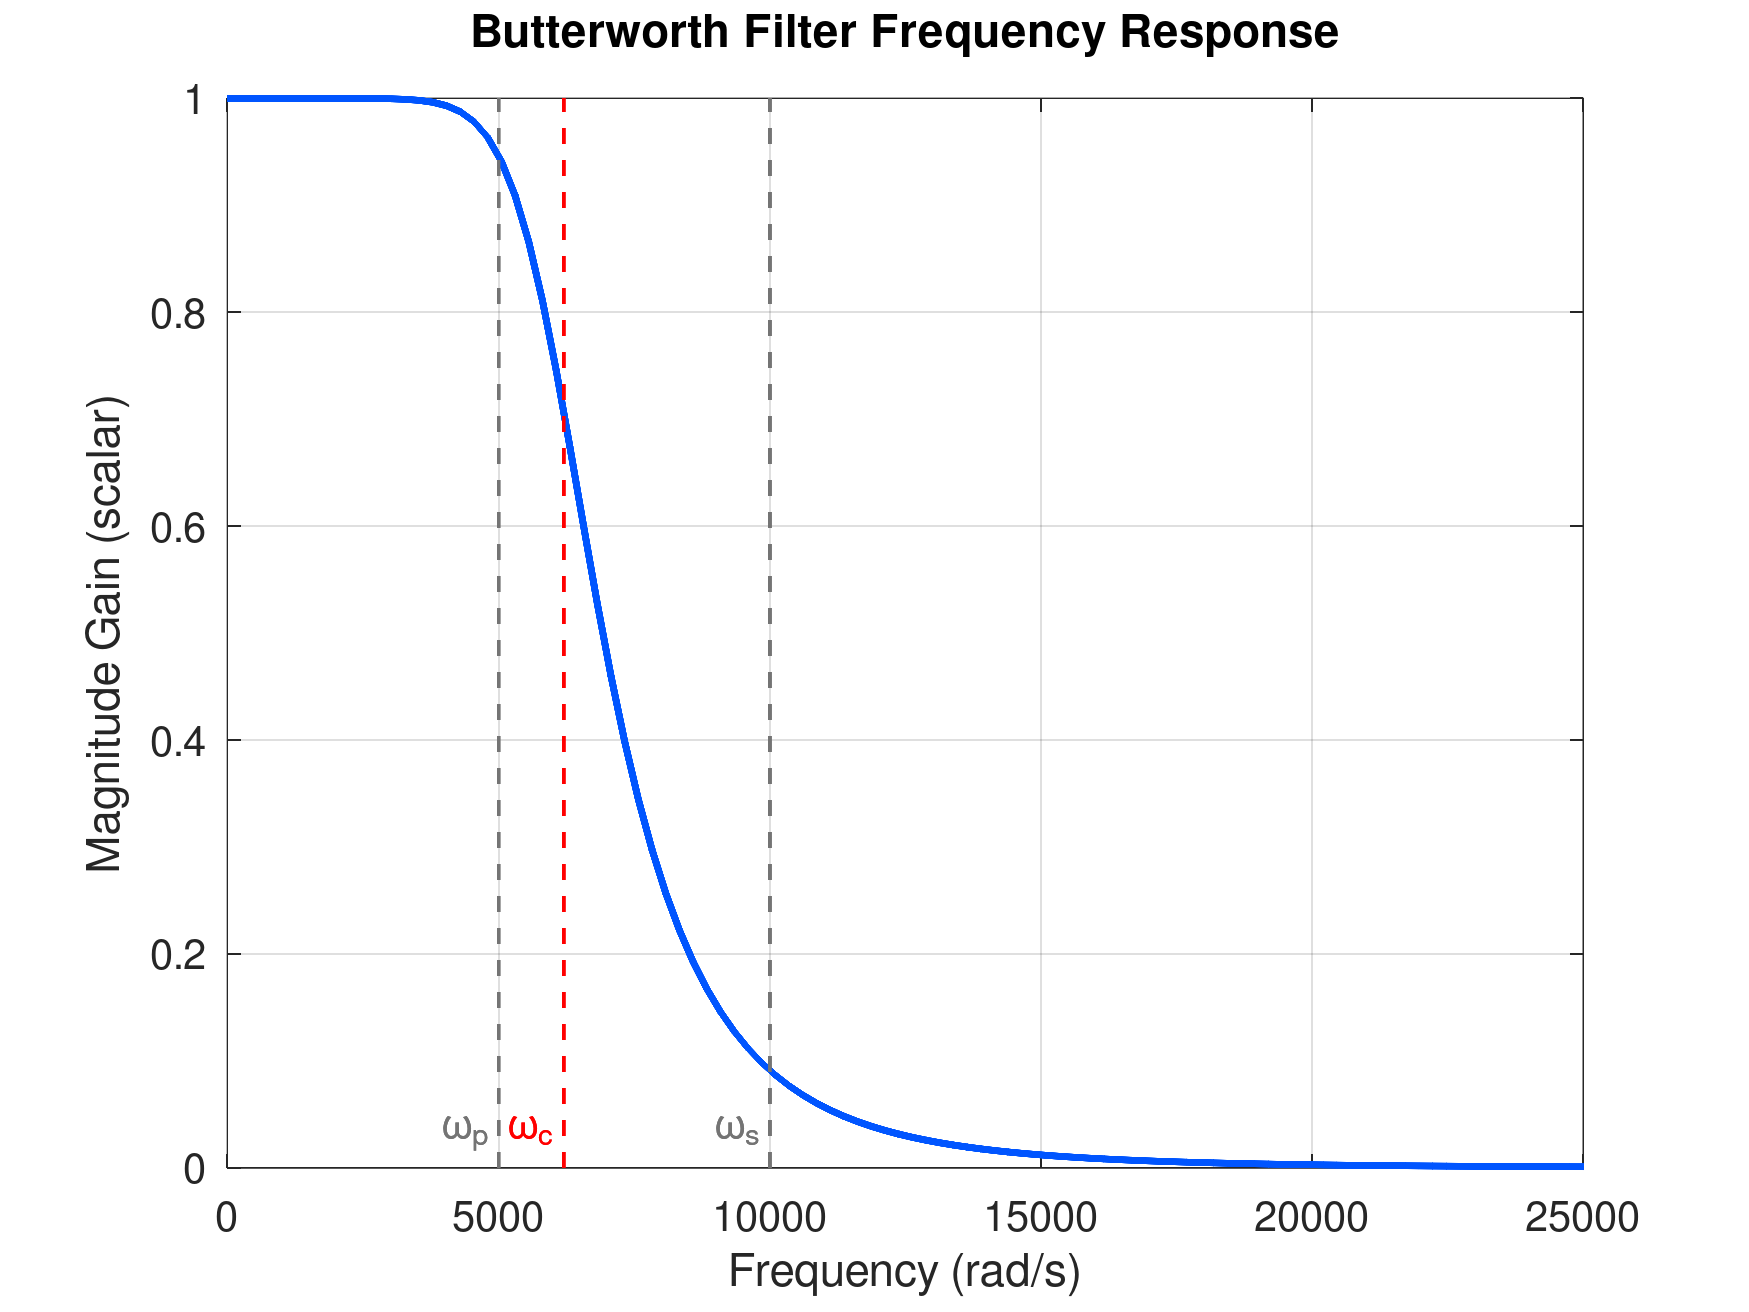
\includegraphics[width=0.7\textwidth]{freq_response.png}
    \caption{Butterworth Filter Frequency Response (Magnitude)}
\end{figure}
\begin{figure}[H]
    \centering
    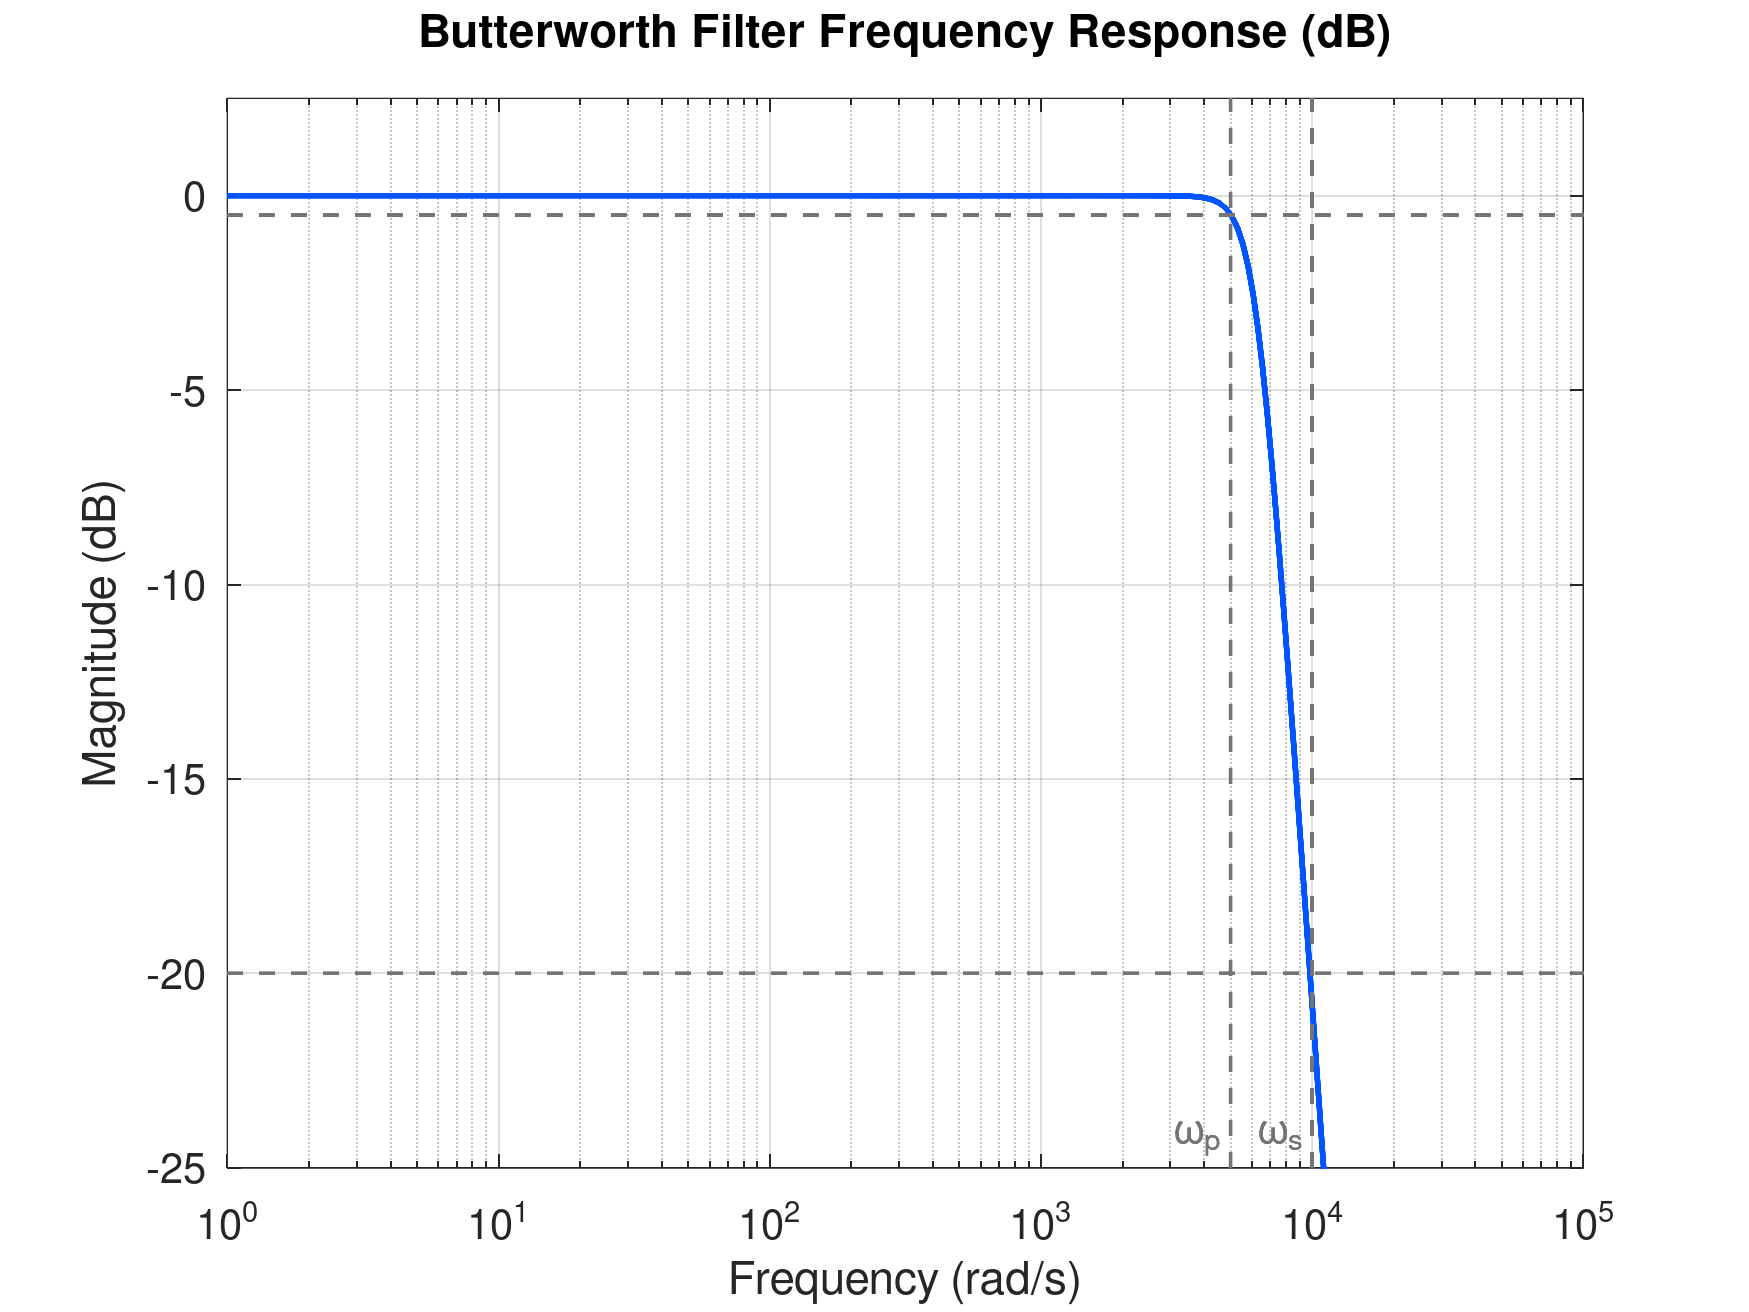
\includegraphics[width=0.7\textwidth]{filter_bode_plot.png}
    \caption{Butterworth Filter Frequency Response (dB)}
\end{figure}


\section*{Verification}
The attenuation at the passband and stopband frequencies is:
\begin{lstlisting}[language=Matlab, caption={Attenuation at Key Frequencies}]
omega_p_dB = 20*log10(abs(H_n(omega_p))); %     = -0.4780 dB
omega_s_dB = 20*log10(abs(H_n(omega_s))); %     = -20.797 dB
\end{lstlisting}
At $\omega_p = 5\text{k rad/s}$, attenuation $= 0.4780$ dB (within spec, $\leq 0.5$ dB).\\
At $\omega_s = 10\text{k rad/s}$, attenuation $= 20.797$ dB (within spec, $\geq 20$ dB).


\section*{Summary}
\begin{itemize}
    \item Designed a 5th-order analog lowpass Butterworth filter to meet given attenuation and frequency specifications.
    \item Calculated the required filter order and cutoff frequency based on design constraints.
    \item Determined pole locations and constructed the transfer function.
    \item Plotted the frequency response to verify filter characteristics.
    \item Verified that the filter meets the specified passband and stopband attenuation requirements.
    \item 
\end{itemize}

\end{document}
